\documentclass{ctexart}
\usepackage{graphicx}
\usepackage{amsmath}
\usepackage{bm}
\begin{document}
	\section{AX=B和它的四个子空间}
	
	\subsection{The geometry of linear equations}
	
	线性代数的基本问题是解决n个未知数的n个等式的方程组
	
	比如:
	
	\[2x − y = 0\]
	
	\[−x + 2y = 3\]
	
	\textbf{从行的角度来看}
	
	如果方程组表示的直线有交点,那么交点就是它们的解
	
	\begin{center}
		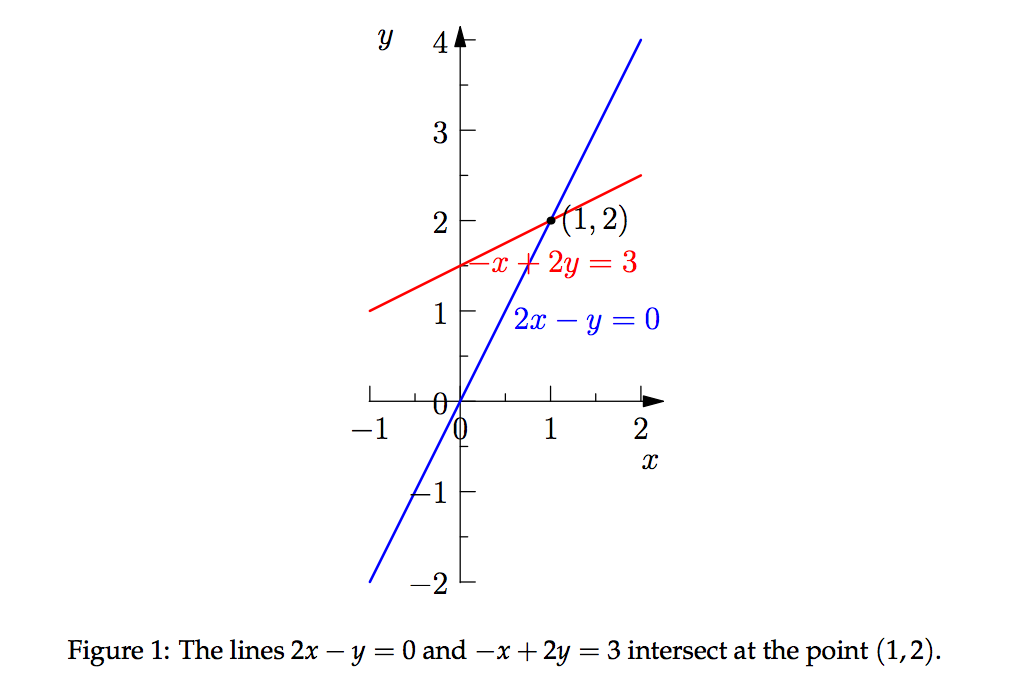
\includegraphics[width=0.8\linewidth]{pic/plot_two_equation}
	\end{center}

	\textbf{从列的角度来看}
	
	通过把方程组的系数变成列向量,可以把方程组写成一个等式
	
	\[x\begin{bmatrix}
	2 \\ -1 
	\end{bmatrix}+ 
	y\begin{bmatrix}
	-1 \\ 2
	\end{bmatrix} = 
	\begin{bmatrix}
	0 \\ 3
	\end{bmatrix}\]
	
	给定两个向量\(\bm{c}, \bm{d}\),和标量x和y,那么\(x\bm{c}+y\bm{d}\)就是向量\(\bm{c}, \bm{d}\)的线性组合
	
	\begin{center}
		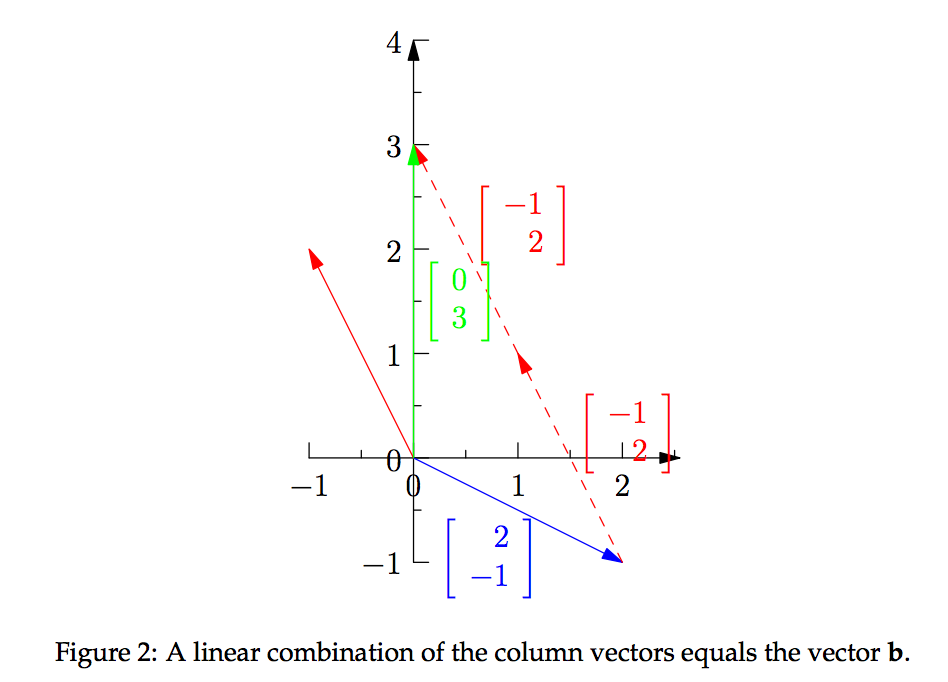
\includegraphics[width=0.8\linewidth]{pic/linear_combination}
	\end{center}

	找到对应的x和y能够使线性组合等于向量\(\bm{b}\)
	
	从列的角度看,对于高维空间的情况更容易想象
	
	\textbf{从矩阵的角度来看}
	
	通过矩阵和向量来表示一个等式
	
	\[\begin{bmatrix}
	2 & -1 \\
	-1 & 2
	\end{bmatrix}
	\begin{bmatrix}
	x \\ y
	\end{bmatrix}=
	\begin{bmatrix}
	0 \\ 3
	\end{bmatrix}\]
	
	矩阵\(A = \begin{bmatrix}
	2 & -1 \\
	-1 & 2
	\end{bmatrix}\)成为系数矩阵,向量\(\bm{x}=\begin{bmatrix}
	x \\ y
	\end{bmatrix}\)是未知向量,得等式
	
	\[A\bm{x = b}\]
	
	则关于等式的解,如果A可逆的话
	
	\[\bm{x} = A^T\bm{b}\]

	\subsection{An overview of key ideas}
	
	\textbf{向量}
	
	在三维空间\(R^3\)中
	
	\[u = \begin{bmatrix}
	1 \\
	-1 \\
	0
	\end{bmatrix}, v = \begin{bmatrix}
	0 \\
	1 \\
	-1
	\end{bmatrix}, w = \begin{bmatrix}
	0 \\
	0 \\
	1
	\end{bmatrix}\]

	\(\bm{u}\)构成空间中的一条直线,\(\bm{v}\)构成空间中的另一条直线,\(\bm{u, v}\)的线性组合构成一个平面,一些向量的所有线性组合构成一个子空间
	
	\textbf{矩阵}
	
	\(\bm{u,v,w}\)的线性组合\(c\bm{u}+d\bm{v}+e\bm{w}\)
	
	\[c\begin{bmatrix}
	1 \\
	-1 \\
	0
	\end{bmatrix} + d\begin{bmatrix}
	0 \\
	1 \\
	-1 
	\end{bmatrix} + e\begin{bmatrix}
	0 \\
	0 \\
	1
	\end{bmatrix} = \begin{bmatrix}
	c \\
	d - c \\
	e - d
	\end{bmatrix}\]
	
	
	创建一个矩阵A,\(\bm{u,v,w}\)是列向量,上述式子可以表示成\(A\bm{x}=b\)的形式
	
	\[A = \begin{bmatrix}
	1 & 0 & 0 \\
	-1 & 1 & 0 \\
	0 & -1 & 1
	\end{bmatrix} \begin{bmatrix}
	c \\
	d \\
	e
	\end{bmatrix} = \begin{bmatrix}
	c \\
	d - c \\
	e - d
	\end{bmatrix}\]
	
	矩阵A乘以向量\(\bm{x} = (\bm{c, d, e})\)
	
	\[A\bm{x}= \begin{bmatrix}
	\bm{u} & \bm{v} & \bm{w}
	\end{bmatrix} \begin{bmatrix}
	c \\
	d \\
	e
	\end{bmatrix} = c\bm{u}+d\bm{v}+e\bm{w}\]
	
	一开始是数字c,d,e分别乘以向量,\(A\bm{x}\)是矩阵的列向量的线性组合,如今是矩阵作用于这些数字,就是矩阵A作用于向量\(\bm{x}\)
	
	
	\subsection{A=LU}
	
	例子:
	
	\[A=\begin{bmatrix}
	2 & 1 & 0 \\
	1 & 2 & 1 \\
	0 & 1 & 2
	\end{bmatrix} = \begin{bmatrix}
	1 & 0 & 0 \\
	1/2 & 1 & 0 \\
	0 & 2/3 & 1
	\end{bmatrix}\begin{bmatrix}
	2 & 1 & 0 \\
	0 & 3/2 & 1 \\
	0 & 0 & 4/3
	\end{bmatrix} = LU\]
	
	LU分解的过程中是不能进行行变换的,L的主对角线上的数都是1
	
	关于A=LU有以下结论:
	
	L与A的下三角矩阵的形式一致,当A的行以0开头,L的行也是一样
	U与A的上三角矩阵的形式一致,当A的列以0开头,U的列也是一样
	
	\subsection{矩阵转置}
	
	\[(A+B)^T = A^T + B^T\]
	
	\[(AB)^T = B^TA^T\]
	
	\[(A^{-1})^T = (A^T)^{-1}\]
	
	\(A\bm{x}\)是A的列的线性组合,而\(\bm{x}^TA^T\)是\(A^T\)的行的线性组合
	
	当A时对称矩阵即\(A=A^T\),能被分解成LDU,且没有发生行变换,那么\(U=L^T\)
	
	
	
	\section{向量空间\(R^n\)}
	
	向量空间\(R^n\),在此向量空间中的向量就有n个实数组成
	
	\textbf{子空间}
	
	一个向量空间包含在另一个向量空间中,叫做该向量的子空间。子空间的向量应该包含零向量
	\textbf{列空间}
	在三维空间\(R^3\)中给予一个矩阵A,则矩阵A的列和列的所有线性组合构成三维空间的一个子空间,也就是列空间C(A).如果\(A=\begin{bmatrix}
	1 & 3 \\
	2 & 3 \\
	4 & 1
	\end{bmatrix}\),那么A的列空间就是在三维空间中穿过原点,且包含A的两个列向量的一个平面

	\begin{thebibliography}{99}
		\bibitem{ref1}Gilbert Strang: introduction to linear algebra
	\end{thebibliography}


\end{document}